\documentclass{article}
\usepackage{iclr2027_conference,times}
\usepackage{amsmath,amssymb,booktabs,graphicx}
\usepackage{pgfplots}
\pgfplotsset{compat=1.18}
\usepackage{multirow}
\usepackage{url}
\usepackage{hyperref}
\hypersetup{hidelinks,pdfauthor={Anonymous},pdftitle={Beyond the IKEA Effect in LLMs: Post-Completion Self-Devaluation}}

\title{Beyond the IKEA Effect in LLMs: Post-Completion Self-Devaluation}
\author{Anonymous authors}

\newcommand{\live}{\textsc{Live}}
\newcommand{\replay}{\textsc{Replay}}
\newcommand{\post}{\textsc{Post}}

\begin{document}
\maketitle

\begin{abstract}
Inference-time search, self-correction, and branch selection increasingly use language models to score their own intermediate generations. Such systems often treat an online score as if it were interchangeable with the score the same model would assign later. We test that assumption with a matched \live{}--\replay{}--\post{} protocol. \live{} records a sentence score on the original writing trajectory; \replay{} reconstructs the same visible prefix in a fresh call; \post{} scores the sentence after the completed output is visible. This decomposes the total retrospective shift into an IKEA-like writer-state component ($R-L$) and a completion-associated component ($P-R$). Across six models with sufficiently developed three-state data, only one has a positive mean IKEA-like shift ($+2.77$ points), while the other five move in the opposite direction. By contrast, four of six show positive post-completion self-devaluation, with mean $P-R$ shifts from $+3.18$ to $+20.06$ points; one model is near zero and one moves oppositely. In the strongest case, about 88\% of the total \live{}--\post{} change appears only after completion. We call this model-dependent pattern the \emph{Gogol effect}. Separate audits show that score-level error and within-output rank stability are distinct: calibration can reduce level error but cannot repair unstable local rankings. Held-out elicitation and temperature controls preserve the main directional result. The implication is diagnostic rather than psychological: online self-scores can be useful control signals, but their temporal stability, ranking geometry, and dependence on future context must be measured rather than assumed.
\end{abstract}

\section{Introduction}
Large language models increasingly evaluate their own intermediate outputs. Agents critique actions before execution, reasoning systems score partial trajectories, and iterative methods use self-evaluation to decide whether to continue, revise, or abandon an answer \citep{madaan2023selfrefine,shinn2023reflexion,lightman2023verify,snell2024testtime}. These methods create an operational assumption that is easy to overlook: a score emitted \emph{during} generation is treated as a proxy for the score that would be available later.

That assumption need not hold. A model may evaluate the same text differently because it is still on the writing trajectory, because a fresh call changes the conversational state, because later text provides evidence unavailable earlier, or simply because its evaluator is noisy. Existing work already shows self-preference, self-attribution, ownership-like biases, and trajectory-dependent confidence in LLMs \citep{panickssery2024recognize,xu2024pride,khullar2026selfattribution,sanzguerrero2026ownership,han2025finece,gai2026premature,yang2026mirage}. The question here is narrower: \emph{what part of the online-to-retrospective discrepancy is associated with leaving the original writing trajectory, and what part appears only after the output is complete?}

The distinction matters because a large \live{}--\post{} gap can invite an IKEA-like interpretation: perhaps the model ``likes'' its own output while producing it and becomes more critical later. We test that interpretation using three evaluation states. \live{} is the score emitted on the original generation trajectory. \replay{} reconstructs the visible prefix through the same sentence in a fresh call. \post{} evaluates that sentence after the full output is available. For a sentence with scores $L$, $R$, and $P$,
\begin{equation}
P-L=(R-L)+(P-R).
\label{eq:decomp}
\end{equation}
Our score is AI-likeness, where higher means less favorable to the generated text. Thus $R-L>0$ is directionally consistent with an IKEA-like writer/self-attribution effect, while $P-R>0$ means the sentence is judged more harshly only after completion. We call the latter operational pattern \emph{post-completion self-devaluation}, or, for memorability, the \emph{Gogol effect}. The name alludes to Nikolai Gogol's famous destruction of much of the second part of \emph{Dead Souls} late in his life \citep{gogolbio}; it is a literary metaphor, not a claim that models experience regret, ownership, or any human mental state.

The central result reverses the motivating story. Across six models with developed three-state data, a positive IKEA-like mean appears in only one model, and is modest. Positive post-completion self-devaluation appears in four, and can be much larger. The strongest case assigns roughly 88\% of its total retrospective shift to $P-R$, not $R-L$. A two-state design would conflate these qualitatively different trajectories.

We make four contributions. First, we introduce a matched \live{}--\replay{}--\post{} diagnostic that separates a writer-state-associated component from a completion-associated component without claiming a hidden-state causal intervention. Second, we show that the IKEA-like explanation is uncommon in our six-model decomposition, while post-completion self-devaluation is recurrent but model-dependent. Third, we separate \emph{level agreement} from \emph{rank reliability}: a calibratable offset is not the same failure as a changed local ordering. Fourth, we stress-test the result with held-out elicitation variants, a temperature control, and an equal-compute rewrite check.

Our endpoint is intentionally narrow: perceived AI-likeness of short factual social posts. It is useful because the same scalar judgment can be elicited online and retrospectively, but it is not a validated probability of human detection and it is not correctness confidence. We therefore do not claim that the observed decomposition generalizes unchanged to mathematical or code verification. Testing that task dependence is an important next step.

\section{Related Work}
\paragraph{Self-evaluation and trajectory-dependent confidence.}
LLMs can provide informative self-estimates under some elicitation schemes \citep{kadavath2022know}, and self-feedback is used in iterative methods such as Self-Refine and Reflexion \citep{madaan2023selfrefine,shinn2023reflexion}. More recent work explicitly studies confidence along a developing trajectory. FineCE uses later text to revise confidence about earlier prefixes \citep{han2025finece}; premature-confidence work links early commitment to flawed reasoning \citep{gai2026premature}; and trajectory-grounding work shows that apparently calibrated confidence can remain weakly tied to the actual reasoning path \citep{yang2026mirage}. Our novelty claim is therefore not that confidence changes over time, but the matched three-state decomposition of the same generated material.

\paragraph{Self-preference and self-attribution.}
LLM judges exhibit evaluator biases even when they correlate with human preferences \citep{zheng2023judge,wang2024fair}. Models can favor outputs from themselves or their model family \citep{liu2024narcissistic,panickssery2024recognize,wataoka2024selfpreference}; self-refinement can amplify self-bias \citep{xu2024pride}; and identical content may be judged more favorably when conversational structure attributes it to the evaluator itself \citep{khullar2026selfattribution,sanzguerrero2026ownership}. These results motivate the IKEA analogy but do not establish that such bias explains a \live{}--retrospective gap.

\paragraph{Inference-time control.}
Selectors, verifiers, and self-correction systems consume model-produced scores and critiques \citep{wang2023selfconsistency,lightman2023verify,snell2024testtime}. Trained systems such as SCoRe target self-correction directly \citep{kumar2025score}. We do not benchmark a general self-correction algorithm; our concern is upstream: whether a score available online preserves the ordering or level that the same scoring rule would produce later.

\section{Three-State Audit}
\subsection{Evaluation states and contrasts}
For model $m$, prompt $q$, and sentence $i$, let $L_{mqi}$, $R_{mqi}$, and $P_{mqi}$ denote \live{}, \replay{}, and \post{} scores. Scores range from 0 (very human-like) to 100 (obviously AI-generated). We use two signed contrasts:
\begin{align}
\Delta^{\mathrm{IKEA}} &= R-L,\\
\Delta^{\mathrm{Gogol}} &= P-R.
\end{align}
Positive $R-L$ means \live{} was more favorable than a fresh prefix-matched replay. Positive $P-R$ means the earlier text is judged more AI-like after the completed response becomes available. These are operational state contrasts, not psychological constructs.

\subsection{Three properties of an online score}
\paragraph{Rank reliability.}
For local selection, the key question is whether \live{} preserves the ordering later assigned by \post{}. We report mean within-output Spearman correlation
\begin{equation}
\mathcal{R}_m=\frac{1}{|Q_m|}\sum_{q\in Q_m}\rho_s(L_{mq\cdot},P_{mq\cdot})
\end{equation}
and non-tied pairwise ordering agreement. This directly matches decisions such as ``which sentence should be revised?''

\paragraph{Level agreement.}
We report bias $\mathbb{E}[L-P]$ and MAE $\mathbb{E}|L-P|$. A stable shift may be correctable without changing ranking. We therefore fit offset-only and affine \live{}$\rightarrow$\post{} mappings with five-fold cross-validation grouped by prompt.

\paragraph{State stability.}
\replay{} asks whether a fresh call given approximately the same visible prefix reproduces the online judgment. Importantly, hosted APIs do not expose hidden activations, and later REPLAY steps contain REPLAY's own earlier score tokens rather than the corresponding LIVE scores. Thus Eq.~\ref{eq:decomp} is algebraically exact, while the causal interpretation of its components is deliberately limited. $R-L$ includes writer-versus-fresh-call differences plus any divergence in prior score-token history; $P-R$ includes completion information plus the retrospective prompting transition.

\subsection{What the audit does not establish}
\post{} is not ground truth. Weak \live{}--\post{} agreement could reflect state sensitivity, a weak retrospective evaluator, or both. The audit is appropriate when a controller intends to substitute an online score for a delayed score from the \emph{same evaluation rule}. External validity requires a separate benchmark with task-specific labels or human judgments. This distinction addresses evaluator reliability directly: our claim is consistency across states, not that the model is an objectively correct judge.

\section{Experimental Design}
\subsection{Probe, prompts, and models}
We froze 110 factual social-writing prompts: 100 English primary prompts and 10 non-English validation prompts. Each asks for a 5--8 sentence social-network post; topics span ten domains. The main English confirmation set contains 40 prompts, four per domain. After every sentence in \live{}, the generating model emits an integer AI-likeness score. \post{} receives the completed clean output with one score placeholder per sentence. \replay{} reconstructs the textual prefix through a target sentence and requests only that sentence's missing score. Exact templates appear in Appendix~\ref{app:protocol}.

We attempted ten models through frozen OpenRouter route identifiers: GPT-5.5, Claude Opus 5, Gemini 3.1 Pro Preview, DeepSeek V4 Flash, DeepSeek V3.2, GPT-OSS-120B, Llama 3.3-70B-Instruct, Qwen3-30B-A3B-Instruct, Ministral 14B, and Gemma 3-12B-IT. All primary calls, including isolated numeric-score calls, used temperature 0.7. Provider routing used OpenRouter automatic routing with fallbacks, a reproducibility limitation we report rather than hide.

\subsection{Confirmation and REPLAY extension}
The original adaptive confirmation used planned looks at $N\in\{40,50,60,70,80,90,100\}$ with familywise $\alpha=.05$. It stopped at $N=40$ when three pre-specified tests crossed the Bonferroni boundary: GPT-5.5 prompt-level mean-score \live{}--\post{} Spearman exceeded a reference $\rho_0=.2$; Gemini's mean $P-L$ exceeded five points; and Gemini's shift exceeded GPT-5.5's by more than five points. The prompt-level statistic correlates, across prompts, each output's mean LIVE score with its mean POST score; this is distinct from the within-output ranking metric above.

Full REPLAY was then collected on all 40 English prompts for GPT-5.5 and Gemini. To broaden the decomposition, four additional models with adequate LIVE/POST coverage and reliable REPLAY parsing were extended adaptively in frozen blocks of four, up to 24 prompts. Because an initial four-prompt pilot had already been inspected, cumulative stopping $p$-values are descriptive; inferential support for positive breadth extensions uses only newly added prompts with Bonferroni correction over the possible future looks. Details are in Appendix~\ref{app:adaptive}.

\subsection{Robustness and downstream check}
Two held-out cohorts vary the scoring surface: original wording/tag, a semantic paraphrase, reverse-coded human-likeness (normalized as $100-n$), and a minimal numeric tag. A separate 10-prompt control runs full \live{}--\replay{}--\post{} at both $T=0$ and $T=.7$ for GPT-5.5 and Gemini. Finally, an equal-compute rewrite check compares rewriting the highest LIVE-scored sentence against rewriting a deterministic random different sentence. Both arms use the same instruction and are evaluated by a fresh POST pass over the corrected document. The exact rewrite prompt and exclusions are in Appendix~\ref{app:rewrite}.

\section{Results}
\subsection{The two-state gap is real but not self-explanatory}
The original confirmation stopped at $N=40$. GPT-5.5 showed positive prompt-level mean-score \live{}--\post{} association ($\rho=.599$, one-sided $p=.00147$ against $\rho_0=.2$). Gemini's mean $P-L$ shift was $+22.83$ points ($p=6.9\times10^{-7}$), exceeding GPT-5.5's shift by $19.02$ points ($p=.00111$). Thus an online score can retain information about a model's later judgment while changing substantially in level. But this two-state result does not identify why it changes.

\subsection{IKEA-like writer-state bias is uncommon}
Table~\ref{tab:decomp} reports the six-model decomposition. Gemini is the only model with a positive mean $R-L$: $+2.77$ points on 40 prompts. The other five means are negative, from $-3.01$ to $-8.40$. In this probe, systematic self-favoring on the original writing trajectory is therefore not the dominant cross-model pattern.

\begin{table}[t]
\centering
\caption{Three-state decomposition. $R-L>0$ is IKEA-like; $P-R>0$ is the Gogol direction. The four breadth-extension sample sizes are adaptive.}
\label{tab:decomp}
\small
\begin{tabular}{lrrr}
\toprule
Model & $N$ & $R-L$ & $P-R$\\
\midrule
GPT-5.5 & 40 & $-3.10$ & $+6.91$\\
Gemini 3.1 Pro & 40 & $+2.77$ & $+20.06$\\
GPT-OSS-120B & 8 & $-6.48$ & $+10.00$\\
DeepSeek V4 Flash & 12 & $-8.40$ & $+3.18$\\
Llama 3.3 70B & 24 & $-3.81$ & $+0.24$\\
Claude Opus 5 & 24 & $-3.01$ & $-2.05$\\
\bottomrule
\end{tabular}
\end{table}

This result does not contradict prior ownership/self-attribution studies: REPLAY is not a direct ownership manipulation. It only shows that the transition from the native writing trajectory to our reconstructed prefix rarely moves in the IKEA-like direction.

\subsection{Post-completion self-devaluation is more frequent and larger}
$P-R$ shows a different pattern. GPT-5.5 and Gemini shift by $+6.91$ and $+20.06$ points on the fixed 40-prompt set ($p=7.8\times10^{-14}$ and $5.8\times10^{-11}$, one-sided tests). For Gemini, $20.06/22.83\approx88\%$ of the total \live{}--\post{} change appears only after completion.

The breadth extension adds two positive cases. GPT-OSS-120B reaches a mean $P-R=+10.00$ at total $N=8$; the four fresh extension prompts cross the sequential correction ($p_{\rm adj}=.021$). DeepSeek V4 Flash reaches $+3.18$ at $N=12$ with fresh-extension $p_{\rm adj}=.040$. Llama remains near zero at the 24-prompt cap ($+0.24$), and Claude moves oppositely ($-2.05$). We therefore do not claim universality. The empirical statement is narrower: positive completion-associated self-devaluation appears in four of six decomposed models and dominates the strongest observed shifts, whereas a positive IKEA-like mean appears in one.

\begin{figure}[t]
\centering
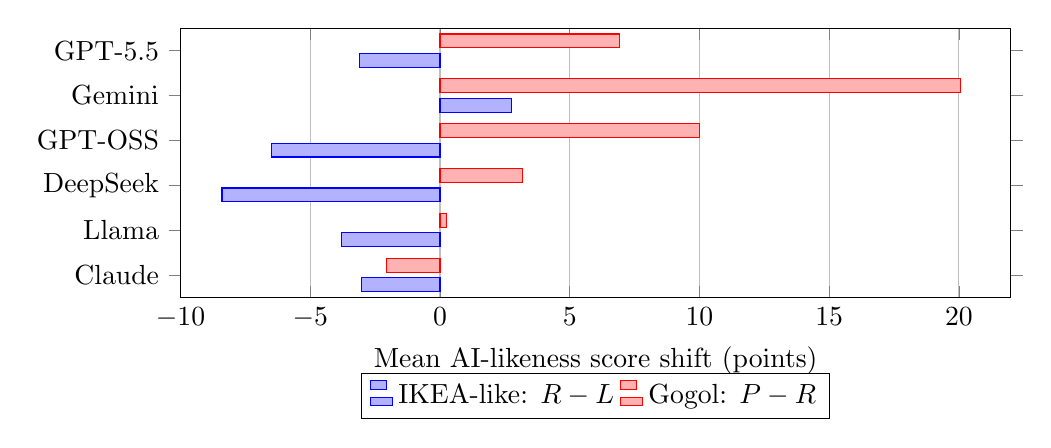
\begin{tikzpicture}
\begin{axis}[
    xbar, width=\linewidth, height=5.0cm,
    xmin=-10,xmax=22,
    symbolic y coords={Claude,Llama,DeepSeek,GPT-OSS,Gemini,GPT-5.5},
    ytick=data,
    xlabel={Mean AI-likeness score shift (points)},
    legend style={at={(0.5,-0.28)},anchor=north,legend columns=2},
    xmajorgrids=true,
    bar width=5pt]
\addplot coordinates {(-3.01,Claude) (-3.81,Llama) (-8.40,DeepSeek) (-6.48,GPT-OSS) (2.77,Gemini) (-3.10,GPT-5.5)};
\addplot coordinates {(-2.05,Claude) (0.24,Llama) (3.18,DeepSeek) (10.00,GPT-OSS) (20.06,Gemini) (6.91,GPT-5.5)};
\legend{IKEA-like: $R-L$,Gogol: $P-R$}
\end{axis}
\end{tikzpicture}
\caption{The writer-state-associated and completion-associated shifts differ qualitatively across models. Error bars and inferential details are reported in Appendix~\ref{app:adaptive}.}
\label{fig:decomp}
\end{figure}

\subsection{Level error and rank reliability are different failures}
Across the ten-model descriptive sweep, mean within-output LIVE--POST Spearman ranges from .329 to .820 while raw MAE ranges from 4.2 to 24.5 points. Claude Opus 5 and GPT-5.5 preserve local retrospective ordering well (mean $\rho=.820$ and $.817$), while Gemini and Qwen3 are much lower ($.345$ and $.329$). Yet Qwen has the smallest raw MAE (4.25), whereas Gemini has the largest (24.47). A model can therefore be close in absolute level while poor at local selection, or shifted in level while preserving ordering.

Five-fold grouped calibration reinforces the distinction. An affine mapping reduces held-out MAE for several models (e.g., Gemini from 24.47 to 20.43; GPT-OSS from 8.63 to 6.87), but any monotone affine correction leaves the within-output ranking unchanged. A controller that thresholds a score may benefit from recalibration; a controller that selects the worst span needs a separate rank audit. Full coverage and calibration tables appear in Appendix~\ref{app:coverage}.

\subsection{Held-out controls preserve the directional result}
A fresh 24-prompt extension repeated LIVE and POST under four semantically matched elicitation schemes for GPT-5.5 and Gemini. All eight model--elicitation mean $P-L$ shifts were positive with prompt-bootstrap 95\% intervals above zero. Averaged across variants within prompt, GPT-5.5 shifted $+5.33$ points and Gemini $+8.61$, with a matched difference of $+3.28$ (95\% CI $[0.72,5.97]$). On the pooled 40 robustness prompts, the matched Gemini-minus-GPT difference is $+4.57$ (95\% CI $[2.05,7.27]$). Rank reliability is more sensitive to the elicitation surface, which is itself an operational warning.

The temperature control addresses a concern that numeric score tokens sampled at $T=.7$ could create the apparent state shift. At $T=0$, GPT-5.5 has $R-L=-1.97$ and $P-R=+7.13$; Gemini has $R-L=-0.01$ and $P-R=+25.27$. Thus the positive post-completion component in these high-coverage models does not require stochastic score-token sampling. Temperature changes the generated prose trajectory too, so the $T=0$ versus $T=.7$ contrast is not a clean causal estimate of temperature itself.

\subsection{Good target ranking is not sufficient for one-shot correction}
The equal-compute rewrite check asks whether a useful LIVE ranking automatically translates into a useful correction policy. It does not. For GPT-5.5 ($N=40$), the guided advantage is $-0.28$ POST-score points; for Gemini, 37 valid pairs yield $+0.27$, with neither paired win-rate test significant. This null is particularly informative for GPT-5.5 because the LIVE target is retrospectively the highest-scored sentence in 72.5\% of outputs and in the top two in 87.5\%. Correctly locating a problematic span is not sufficient for this one-shot rewrite operator to improve the whole document. Gemini's much weaker LIVE--POST rank reliability also makes its granular POST delta a noisier outcome, so the GPT-5.5 null is the cleaner diagnostic. We do not generalize either result to stronger multi-turn self-correction methods.

\section{Discussion}
\paragraph{The original IKEA story is too simple.}
The motivating two-state pattern could be narrated as self-favoring while writing. REPLAY changes that conclusion. In five of six decomposed models, $R-L$ is negative, while four show positive $P-R$. Gemini can exhibit both: a small IKEA-like writer-state component followed by a much larger completion-associated component. GPT-OSS and DeepSeek V4 move in the opposite direction at REPLAY and then reverse after completion. A simple LIVE--POST difference hides these trajectories.

\paragraph{Why completion can matter.}
A later sentence can reveal repetition, formulaic structure, inconsistency, or a global pattern that changes how an earlier sentence looks. This is especially plausible for a holistic stylistic property such as AI-likeness. For locally verifiable mathematical or code steps, future context may matter less, and the decomposition may look different. The current results therefore motivate, rather than settle, generalization to objective reasoning.

\paragraph{Implications for inference-time control.}
The practical lesson is not that POST is superior. POST has information unavailable online. Instead, a controller should audit the property it actually consumes. Thresholding requires level stability or validated recalibration; local selection requires ordering stability; and any system comparing online and delayed scores should test whether later context creates a systematic state shift. A single scalar ``calibration'' summary can obscure these distinct failure modes.

\paragraph{Future work.}
Three extensions are especially important. First, open-weight models would permit stronger replay interventions that control token history and inspect hidden-state effects. Second, the protocol should be applied to objective endpoints---mathematical correctness, code execution, or process-verifier scores---where future-context dependence may differ from stylistic judgments. Third, live-score diagnostics should be integrated with stronger multi-turn correction policies to distinguish failure of target selection from failure of the correction operator.

\section{Limitations}
The endpoint is perceived AI-likeness of short social-writing outputs, not correctness. No human judgments enter the reported score endpoint, so the study establishes state-indexed consistency among model scores, not human-valid detection ability. REPLAY reconstructs visible text but cannot hold hidden activations, provider state, or prior score-token history fixed. Six models have sufficiently developed three-state data for the cross-model effect comparison, and four of those use adaptive breadth-extension sample sizes. Low protocol adherence for several other models can introduce survivorship bias in descriptive reliability comparisons. The robustness follow-up was frozen after an earlier cohort had been inspected, and the temperature control contains only 10 prompts. Hosted model routes can also change over time. These limitations bound the claim to a reproducible operational pattern in the tested model/serving configurations rather than a prevalence estimate over all LLMs.

\section{Conclusion}
A large discrepancy between online and retrospective self-scores need not be an IKEA-like ownership bias. In our six-model decomposition, only one model has a positive mean writer-state-associated shift, whereas four show positive post-completion self-devaluation. In the strongest case, roughly 88\% of the total retrospective shift appears only after the completed output is visible. We call this model-dependent pattern the Gogol effect. More generally, live self-scores should be treated as state-dependent control signals: their level, local ranking, and temporal stability require separate validation before they are used for search, selection, or self-correction.

\section*{AI Use Disclosure}
Generative AI tools assisted with manuscript drafting and editing, literature discovery, experimental workflow organization, code development and debugging, and discussion of experimental design and statistical analysis. AI tools were also part of the experimental subject matter: the reported synthetic text and model-produced scores were generated by the evaluated language models. The author made the final methodological decisions, executed and inspected the experiments, verified the reported numerical results and citations, determined the interpretations and conclusions, and takes full responsibility for the submission.

\section*{Ethics Statement}
The quantitative experiments use synthetic prompts, model-generated text, and model-produced scores. No private or personally identifying human data contribute to the reported estimates. The phrase ``average human reader'' is part of the model-scoring instruction and should not be interpreted as a measurement of actual human opinion. The study compares properties of model-generated control signals and does not rank demographic or protected groups.

\begin{thebibliography}{99}
\bibitem[Encyclopedia of Russian History(2004)]{gogolbio} \emph{Encyclopedia of Russian History}. Gogol, Nikolai Vasilievich. Macmillan Reference USA, 2004.
\bibitem[Norton et~al.(2012)Norton, Mochon, and Ariely]{norton2012ikea} Michael I. Norton, Daniel Mochon, and Dan Ariely. The IKEA effect: When labor leads to love. \emph{Journal of Consumer Psychology}, 22(3):453--460, 2012.
\bibitem[Han et~al.(2025)Han et~al.]{han2025finece} Jinyi Han et~al. Mind the Generation Process: Fine-Grained Confidence Estimation During LLM Generation. arXiv:2508.12040, 2025.
\bibitem[Gai et~al.(2026)Gai et~al.]{gai2026premature} Jingchu Gai et~al. Understanding and Mitigating Premature Confidence for Better LLM Reasoning. arXiv:2605.24396, 2026.
\bibitem[Sanz-Guerrero et~al.(2026)Sanz-Guerrero, Mager, and von der Wense]{sanzguerrero2026ownership} Mario Sanz-Guerrero, Manuel Mager, and Katharina von der Wense. Large Language Models Are Overconfident in Their Own Responses. arXiv:2606.03437, 2026.
\bibitem[Yang et~al.(2026)Yang et~al.]{yang2026mirage} Jisoo Yang et~al. The Mirage of Calibrated Confidence: Trajectory-Independence of Verbalized Confidence in Vision-Language Models. arXiv:2609.18453, 2026.
\bibitem[Khullar et~al.(2026)Khullar et~al.]{khullar2026selfattribution} Dipika Khullar, Jack Hopkins, Rowan Wang, and Fabien Roger. Self-Attribution Bias: When AI Monitors Go Easy on Themselves. arXiv:2603.04582, 2026.
\bibitem[Xu et~al.(2024)Xu et~al.]{xu2024pride} Wenda Xu et~al. Pride and Prejudice: LLM Amplifies Self-Bias in Self-Refinement. \emph{ACL}, 2024.
\bibitem[Liu et~al.(2024)Liu, Moosavi, and Lin]{liu2024narcissistic} Yiqi Liu, Nafise Sadat Moosavi, and Chenghua Lin. LLMs as Narcissistic Evaluators: When Ego Inflates Evaluation Scores. \emph{Findings of ACL}, 2024.
\bibitem[Panickssery et~al.(2024)Panickssery, Bowman, and Feng]{panickssery2024recognize} Arjun Panickssery, Samuel R. Bowman, and Shi Feng. LLM Evaluators Recognize and Favor Their Own Generations. \emph{NeurIPS}, 2024.
\bibitem[Wataoka et~al.(2024)Wataoka, Takahashi, and Ri]{wataoka2024selfpreference} Koki Wataoka, Tsubasa Takahashi, and Ryokan Ri. Self-Preference Bias in LLM-as-a-Judge. arXiv:2410.21819, 2024.
\bibitem[Kadavath et~al.(2022)Kadavath et~al.]{kadavath2022know} Saurav Kadavath et~al. Language Models (Mostly) Know What They Know. arXiv:2207.05221, 2022.
\bibitem[Madaan et~al.(2023)Madaan et~al.]{madaan2023selfrefine} Aman Madaan et~al. Self-Refine: Iterative Refinement with Self-Feedback. \emph{NeurIPS}, 2023.
\bibitem[Shinn et~al.(2023)Shinn et~al.]{shinn2023reflexion} Noah Shinn et~al. Reflexion: Language Agents with Verbal Reinforcement Learning. \emph{NeurIPS}, 2023.
\bibitem[Zheng et~al.(2023)Zheng et~al.]{zheng2023judge} Lianmin Zheng et~al. Judging LLM-as-a-Judge with MT-Bench and Chatbot Arena. \emph{NeurIPS}, 2023.
\bibitem[Wang et~al.(2024)Wang et~al.]{wang2024fair} Peiyi Wang et~al. Large Language Models are not Fair Evaluators. \emph{ACL}, 2024.
\bibitem[Wang et~al.(2023)Wang et~al.]{wang2023selfconsistency} Xuezhi Wang et~al. Self-Consistency Improves Chain of Thought Reasoning in Language Models. \emph{ICLR}, 2023.
\bibitem[Snell et~al.(2024)Snell et~al.]{snell2024testtime} Charlie Snell et~al. Scaling LLM Test-Time Compute Optimally can be More Effective than Scaling Model Parameters. arXiv:2408.03314, 2024.
\bibitem[Lightman et~al.(2023)Lightman et~al.]{lightman2023verify} Hunter Lightman et~al. Let's Verify Step by Step. arXiv:2305.20050, 2023.
\bibitem[Kumar et~al.(2025)Kumar et~al.]{kumar2025score} Aviral Kumar et~al. Training Language Models to Self-Correct via Reinforcement Learning. \emph{ICLR}, 2025.
\end{thebibliography}

\appendix
\section{Frozen Prompt and Execution Protocol}
\label{app:protocol}
The frozen bank contains 100 English primary prompts and 10 non-English validation prompts. The English main subset is balanced at four prompts per domain. The generated-post contract is 5--8 sentences. The scoring scale is 0 (very human-like) to 100 (obviously AI-generated), estimating how likely an average human reader would be to think the sentence was AI-generated. The frozen system instruction was: ``Follow the user's writing task and formatting instructions exactly. Return only the requested output.''

The main API run was executed on September 7, 2026. All primary conditions used temperature 0.7. Output caps were 4096 tokens for LIVE and POST and 1024 for each REPLAY call; no explicit input truncation was applied. Seed was 20260907, with up to 20 global workers, at most one worker per model, and three retries. Provider policy was OpenRouter automatic routing with fallbacks enabled.

\paragraph{Common user prefix.} Every LIVE, POST, and REPLAY user message begins with the original writing task followed by the same scoring instruction. LIVE then appends: ``Produce the requested text now and follow the scoring instruction exactly.''

\paragraph{POST template.} POST receives the complete frozen text with one \texttt{<AI SCORE: ?>} placeholder per sentence and the instruction: ``The requested text has already been produced below. Assess that exact completed text without rewriting it. There are N placeholders, one for each sentence. Return exactly the same number of \texttt{<AI SCORE: n>} tags, one per line and in sentence order. Do not repeat, continue, or rewrite the text.''

\paragraph{REPLAY template.} REPLAY receives only the text prefix through the target sentence, with the final score replaced by \texttt{<AI SCORE: ?>}. It is instructed: ``Continue the assessment for the text below. The only missing content is the single final \texttt{<AI SCORE: ?>}. Do not repeat, continue, or rewrite the text. Replace that placeholder with the score required by the scoring instruction and return only \texttt{<AI SCORE: n>}.'' Later REPLAY steps include earlier REPLAY scores rather than corresponding LIVE scores.

\section{Coverage and Calibration}
\label{app:coverage}
\begin{table}[h]
\centering\small
\caption{English paired LIVE--POST coverage and reliability.}
\begin{tabular}{lrrrr}
\toprule Model & $Q$ & mean $\rho$ & Pair & MAE\\\midrule
Claude Opus 5 & 37 & .820 & .866 & 7.0\\
GPT-5.5 & 40 & .817 & .864 & 5.8\\
Llama 3.3 70B & 40 & .685 & .802 & 7.8\\
GPT-OSS-120B & 40 & .640 & .792 & 8.6\\
Ministral 14B & 12 & .521 & .719 & 5.1\\
DeepSeek V4 & 32 & .504 & .723 & 9.7\\
Gemma 3 12B & 35 & .491 & .705 & 15.8\\
DeepSeek V3.2 & 18 & .444 & .690 & 16.5\\
Gemini 3.1 Pro & 40 & .345 & .659 & 24.5\\
Qwen3 30B & 39 & .329 & .649 & 4.2\\\bottomrule
\end{tabular}
\end{table}
Protocol failures were predominantly failures to obey the exact sentence-plus-score contract. Missing scores were not imputed. Because adherence may correlate with prompt difficulty or output complexity, low-coverage estimates can suffer survivorship bias and should not be read as controlled head-to-head comparisons.

\begin{table}[h]
\centering\small
\caption{Five-fold prompt-grouped LIVE$\rightarrow$POST MAE.}
\begin{tabular}{lrrr}\toprule Model&Raw&Offset&Affine\\\midrule
Qwen3 30B&4.25&4.47&3.73\\
GPT-5.5&5.79&5.49&5.49\\
Claude Opus 5&7.02&6.64&6.32\\
Llama 3.3 70B&7.84&8.41&7.17\\
GPT-OSS-120B&8.63&7.47&6.87\\
DeepSeek V4&9.65&9.86&9.16\\
Gemini 3.1 Pro&24.47&20.07&20.43\\\bottomrule
\end{tabular}
\end{table}
These mappings target agreement with the model's own POST scores, not calibration to human probabilities.

\section{Adaptive REPLAY Breadth Extension}
\label{app:adaptive}
The breadth cohort was Claude Opus 5, DeepSeek V4 Flash, GPT-OSS-120B, and Llama 3.3-70B-Instruct. Qwen3 and Gemma 3 were excluded because earlier REPLAY calls frequently violated the single-score contract; DeepSeek V3.2 and Ministral had substantially lower usable LIVE/POST coverage. An already-inspected four-prompt REPLAY pilot was retained in effect-size estimates. New prompts were then added in frozen blocks of four up to 24 per model. Models stopped receiving API calls once an exploratory cumulative one-sided test for $P-R>0$ crossed .05. Because the stopping rule was chosen after inspection of the four-prompt pilot, cumulative stopping $p$-values are descriptive. For inferential support, the fresh extension prompts were additionally tested with a Bonferroni correction over the five possible future looks. GPT-OSS-120B crosses at total $N=8$ ($p_{\rm adj}=.021$), DeepSeek V4 Flash at $N=12$ ($p_{\rm adj}=.040$), while Claude and Llama continue to the 24-prompt cap.

For the fixed 40-prompt set, Gemini's $R-L$ mean is $+2.772$ (one-sided $t$ test $p=.0102$; Wilcoxon $p=.0292$) and GPT-5.5's is $-3.103$ (positive-direction $p=.9995$). Their $P-R$ means are $+20.061$ and $+6.914$, respectively. Descriptive 95\% intervals at the breadth cap are $[-4.10,4.58]$ for Llama's $P-R$ and $[-4.15,0.06]$ for Claude's.

\section{Equal-Compute Rewrite Check}
\label{app:rewrite}
Each arm receives the original writing task, the full frozen generated text, and the target sentence. The exact instruction is: ``Rewrite only the TARGET SENTENCE so that an average human reader would be less likely to think it was AI-generated. Preserve its intended meaning and factual content, keep it as one sentence, and make it fit naturally into the frozen text. Do not rewrite any other sentence. Return only the replacement sentence, with no score, label, explanation, quotation marks around the whole answer, or additional text.'' The replacement is spliced into the frozen document and a fresh POST call scores every sentence. The outcome is the corrected document's mean POST score.

GPT-5.5 has 40 valid pairs. Gemini has 37: three pairs were excluded solely because one rewrite violated the strict one-line/one-sentence parser (random arm on one prompt, guided arm on one prompt, and random arm on one prompt). No exclusion depended on the resulting score. The corresponding one-sided Wilcoxon $p$-values are .677 and .392.

\section{Held-Out Robustness Details}
A 16-prompt cohort collected LIVE, POST, and preselected REPLAY under four elicitation variants. A separate 24-prompt follow-up, frozen after the first cohort was inspected, collected all 192 LIVE and 192 POST cells. No successfully completed cell was regenerated because of its observed score. On the fresh 24 prompts, mean $P-L$ shifts for GPT-5.5/Gemini were: original $6.56/8.93$, paraphrase $2.95/6.11$, reverse-coded $1.21/6.24$, and minimal tag $10.61/13.16$. The initial 16-prompt REPLAY cohort also preserved the qualitative decomposition: $P-R$ exceeded $R-L$ in all eight model--elicitation cells.

The 10-prompt held-out temperature control produced the following prompt-mean decomposition: at $T=0$, GPT-5.5 $P-L=+5.17$ (95\% bootstrap CI $[1.57,9.88]$), $R-L=-1.97$, $P-R=+7.13$; Gemini $P-L=+25.26$ ($[16.80,33.81]$), $R-L=-0.01$, $P-R=+25.27$. At $T=.7$, GPT-5.5 gives $+1.95$, $-3.72$, $+5.67$, and Gemini $+13.87$, $-1.63$, $+15.50$, respectively.

\section{Reproducibility Package}
The anonymous supplementary archive contains the frozen prompt bank, manifests, route identifiers, stored outputs, derived score tables, REPLAY and correction artifacts, robustness and temperature-control runs, the adaptive cross-model extension with every interim look, analysis scripts, and deterministic expected outputs. Analyses can be reproduced from the frozen outputs without provider credentials. Exact regeneration of hosted model outputs is not guaranteed because model serving and provider routing are external dependencies.

\end{document}
